\chapter{Many-body basics and wave function expansion methods}\label{ch:many_body}

The goal of many-body quantum mechanics is to solve
the $A$-body time-independent Sch\"{o}dinger equation.
This requires, among other things, the construction of a set of states that span
the $A$-body Hilbert space.
For distinguishable particles, taking a set of single-particle states $\ket{p}$
and building $A$-body product states $\ket{p_1}\ldots\ket{p_A}$ would be a reasonable approach.
However, the wave function of a system of $A$ nucleons,
which are indistinguishable fermions,
must be antisymmetric under the exchange of any two particle labels.
The explicit antisymmetrization of states going from naive product states
quickly becomes unwieldy with growing $A$.

Second quantization offers an alternative that bakes the required antisymmetry
into the formalism.
This formalism is the basis for a class of many-body methods
called wave function expansion methods, which includes the IM-SRG.\@
These methods have the benefit that,
instead of scaling combinatorially in $A$ like exact diagonalization approaches,
they scale polynomially,
taking advantage of knowledge of a good approximate solution to the ground state
to reduce the task to finding corrections to this zeroth-order ansatz.
In this chapter, we introduce the basics of second quantization and normal ordering,
focusing on the case of fermions.
Then we discuss some of the more traditional wave function expansion methods
before discussing the IM-SRG in detail in the next chapter.

\section{Second quantization}\label{sec:second_quantization}

To consider second quantization, one starts by constructing the Fock space,
the direct sum of all $A$-body antisymmetric Hilbert spaces.
As a concrete example, for the zero-, one-, and two-body Hilbert spaces, we have the bases
\begin{align}
  A = 0 & \rightarrow \ket{0}\,, \\
  A = 1 & \rightarrow \{\ket{p}\}\,, \\
  A = 2 & \rightarrow \left\{\frac{\ket{p}_{1}\ket{q}_{2} - \ket{q}_{1}\ket{p}_2}{\sqrt{2}} \, \Big| \, q > p \right\}\,.
\end{align}
These states (and many more) are all in the Fock space,
related to one another via field operators.

The field operators are particle creation and annihilation operators
that connect states in the $A$-body antisymmetric Hilbert space
to states in the $A+1$-body and $A-1$-body antisymmetric Hilbert spaces.
The creation operator \crea{p} creates a particle in the single-particle state $\ket{p}$.
Operating on an $A$-body state with it creates an $A+1$-body state
with an additional particle in state $\ket{p}$,
\begin{equation}
  \crea{p} \ket{p_1 \ldots p_{A}}_a = (1 - n_{p}) \ket{p p_1 \ldots p_{A}}_a\,,
\end{equation}
where we have explicitly denoted that the states are antisymmetrized.
Here, $n_p$ is the occupation number of state $\ket{p}$ in the $A$-body state,
which for fermions, due to the Pauli exclusion principle, can only be 0 or 1.
Attempting to create a second particle in an already occupied state annihilates the state.

The annihilation operator \annih{p} annihilates a particle in the single-particle state $\ket{p}$.
Operating on an $A$-body state with it creates an $A-1$-body state
with a particle in state $\ket{p}$ removed,
\begin{equation}
  \annih{p} \ket{p p_2 \ldots p_A}_a = n_p \ket{p_2 \ldots p_A}_a\,.
\end{equation}
If no particle with the single-particle state $\ket{p}$ exists in the state,
the annihilation operator annihilates the state.

With the field operators, an antisymmetric $A$-body state can very efficiently be written as
\begin{equation}
  \ket{p_1 p_2 \ldots p_A}_a = \crea{p_1} \crea{p_2} \ldots \crea{p_A} \ket{0}\,.
\end{equation}
This antisymmetrized product of $A$ particles in $A$ unique single-particle states
is frequently referred to as a Slater determinant,
owing to the fact that it can be, in its explicitly antisymmetrized form,
written as an appropriately normalized determinant~\cite{Slat29sladet}.

Since these states should be antisymmetric under exchange of particle indices, that is,
\begin{equation}
  \ket{p_1 p_2 \ldots p_A}_a = - \ket{p_2 p_1 \ldots p_A}_a\,,
\end{equation}
the creation and annihilation operators must anti-commute with themselves,
\begin{align}
  \anticomm{\crea{p}}{\crea{q}} = 0\,,\\
  \anticomm{\annih{p}}{\annih{q}} = 0\,.
\end{align}
Similarly, one can arrive at the anti-commutation relation
between creation and annihiliation operators,
\begin{equation}
  \anticomm{\annih{p}}{\crea{q}} = \delta_{pq}\,.
\end{equation}

With this formalism in place,
we are now in a position to discuss the representation of many-body operators
in the Fock space.
Operators are classified as $A$-body operators if they can at most couple $A$ particles.
We have used this language frequently so far,
but we make it very precise in the following discussion.

Zero-body operators are simple scalars,
\begin{equation}
  \zerobodyop{O} = o\,.
\end{equation}
They have, among other things, in general a non-zero vacuum expectation value.

One-body operators are of the form
\begin{equation}\label{eq:onebody_op_definition}
  \onebodyop{O} = \sum_{pq} \onebodyop{O}_{pq} \crea{p} \annih{q}\,,
\end{equation}
where $\onebodyop{O}_{pq}$ are the matrix elements of $\onebodyop{O}$.
One-body operators have two useful properties.
First, their vacuum expectation value is 0:
\begin{equation}
  \braket{0 | \onebodyop{O} | 0} = 0\,.
\end{equation}
Second, they do not contribute to processes
where the incoming (bra) and outgoing (ket) states differ
in more than one single-particle state.
Some examples of one-body operators are the kinetic energy and an external potential.

Two-body operators are of the form
\begin{equation}
  \twobodyop{O} = \frac{1}{{(2!)}^2} \sum_{pqrs} \twobodyop{O}_{pqrs} \crea{p} \crea{q} \annih{s} \annih{r}\,.\label{eq:twobody_op_definition}
\end{equation}
Here $\twobodyop{O}_{pqrs}$ is an antisymmetrized matrix element, with the property
\begin{equation}
  \twobodyop{O}_{pqrs} = - \twobodyop{O}_{qprs} = - \twobodyop{O}_{pqsr} = \twobodyop{O}_{qpsr}\,.
\end{equation}
We note that in Eq.~\ref{eq:twobody_op_definition}
the order of the annihilation operators is reversed
relative to the indices on the matrix element.
The indices $p$ and $r$ and the indices $q$ and $s$ are ``paired,''
and the product of creation and annihilation operators is structured
such that the pairs are nested inside of eachother,
not adjacent to eachother.
However, by the antisymmetry of the matrix elements,
the matrix element for one pairing determines it
for all other pairings of the same creation and annihilation operators.
Two-body operators have the properties
\begin{align}
  \braket{0 | \twobodyop{O} | 0} & = 0\,,\\
  \braket{p | \twobodyop{O} | q} & = 0\,,
\end{align}
and they do not contribute to processes where incoming and outgoing states
differ in more than two single-particle states.
A typical example of a two-body operator is any pairwise interaction,
such as the Coulomb interaction or NN nuclear forces.

Three-body operators are of the form
\begin{equation}\label{eq:threebody_op_definition}
  \threebodyop{O} = \frac{1}{{(3!)}^2} \sum_{pqrstu} \threebodyop{O}_{pqrstu} \crea{p} \crea{q} \crea{r} \annih{u} \annih{t} \annih{s}\,.
\end{equation}
Here, $\threebodyop{O}_{pqrstu}$ are also antisymmetrized matrix elements, with the property
\begin{equation}
  \threebodyop{O}_{pqrstu} = {(-1)}^{\sigma_1}{(-1)}^{\sigma_2}\threebodyop{O}_{\sigma_1(pqr)\sigma_2(stu)}\,,
\end{equation}
where $\sigma_1$ and $\sigma_2$ are permutations
and the ${(-1)}^{\sigma}$ prefactors account for the signs of the permutations.
Three-body operators have the properties
\begin{align}
  \braket{0 | \threebodyop{O} | 0} & = 0\,,\\
  \braket{p | \threebodyop{O} | q} & = 0\,, \\
  \braket{p q| \threebodyop{O} |r s} & = 0\,,
\end{align}
and they do not contribute to processes where incoming and outgoing states
differ in more than three single-particle states.
Examples of three-body operators are 3N nuclear forces.
These definitions can be generalized to get the general representation of any $A$-body operator,
and the properties follow analogously.

\section{Normal ordering}

A product of creation and annihilation operators is in normal order
if all creation operators appear to the left of all annihilation operators.
The normal ordering operation on $c A$,
where c is a scalar coefficient and $A$ is a product of creation and annihilation operators,
can be written as
\begin{equation}
  \nogen{c A} = {(-1)}^{\sigma} c \sigma(A)\,
\end{equation}
where $\sigma$ is a permutation that rearranges the product $A$ into normal order.
This rearrangement is not unique,
but, since each change in the permutation is accompanied by a change in the exchange prefactor,
all normal-ordered products resulting from different permutations used in normal ordering
are equivalent.
Also, note that in general $\nogen{A} \neq A$,
since anti-commuting creation and annihilation operators past eachother
will leave a residual $\delta_{pq}$ from their anti-commutation relation.

\subsection{General properties}\label{sec:normal_ordering_properties}

Suppose the product of creation and annihilation operators $A$
contains $p$ creation operators and $q$ annihilation operators.
Then, unless $p$ and $q$ are both 0,
$\nogen{A}$ has a vacuum expectation value of 0.
Additionally, $\nogen{A}$ does not contribute to processes
where the incoming state has less than $q$ particles
or the outgoing state has less than $p$ particles.

We are now interested in considering products of normal-ordered products
of creation and annihilation operators.
Ultimately, we will use Wick's theorem to systematically evaluate these products~\cite{Wick50wickthm}.
To introduce the theorem, we first need to introduce the notion of a Wick contraction,
which for adjacent operators $\alpha$ and $\beta$ is defined as
\begin{equation}
  \acontraction{}{\alpha}{}{\beta}
  \alpha \beta = \alpha \beta - \nogen{\alpha \beta}\,.
\end{equation}
The value of the contraction is the vacuum expectation value of $\alpha \beta$.
Note that for two operators that are already in normal order their contraction vanishes.
This provides an alternative definition of normal ordering,
namely a product of two operators is in normal order
if its vacuum expectation value is 0
and so its contraction vanishes.
This leads to an extension of normal ordering
that works for many different vacuum choices,
including multi-reference vacuums
which we don't consider any further in this work~\cite{Kutz97mrno}.

We are now equipped to use Wick's theorem
to rewrite a general product of creation and annihilation operators
in terms of sums of normal-ordered products and contractions:
\begin{equation}\label{eq:wicks_theorem}
  \begin{split}
    ABCDEF\ldots =& \nogen{ABCDEF\ldots} \\
    & + \acontraction{}{A}{}{B} AB \,\nogen{CDEF\ldots} - \acontraction{}{A}{}{C} AC \,\nogen{BDEF\ldots} + \text{singles}\\
    &+ \left(\acontraction{}{A}{}{B} AB \acontraction{}{C}{}{D} CD
    - \acontraction{}{A}{}{C} AC \acontraction{}{B}{}{D} BD
    + \acontraction{}{A}{}{D} AD \acontraction{}{B}{}{C} BC\right) \, \nogen{EF\ldots} + \text{doubles} \\
    &+ \cdots + \text{full contractions}\,.
  \end{split}
\end{equation}
The minus signs arise due to the fact that in order to simplify the contraction
and pull it out of the normal-ordered product,
we must anti-commute the contracted operators such that they are adjacent.

The generalized Wick's theorem states that
for a product of two normal-ordered products of creation and annihilation operators,
$A=\nogen{A_1 A_2 \ldots A_N}$ and $B=\nogen{B_1 B_2 \ldots B_M}$,
the resulting expression in terms of normal-ordered products
is the sum of all normal-ordered terms with 0 to $\text{min}(N, M)$ contractions
between the operators in $A$ and $B$, that is,
\begin{equation}\label{eq:gen_wicks_theorem}
  \begin{split}
    \nogen{A_1 A_2 \ldots A_N} \nogen{B_1 B_2 \ldots B_M} = &
    \nogen{A_1 A_2 \ldots A_N B_1 B_2 \ldots B_M} \\
    & + {(-1)}^{N-1} \acontraction{}{A_1}{}{B_1} A_1 B_1 \nogen{A_2 \ldots A_N B_2 \ldots B_M} \\
    & + {(-1)}^{N-2} \acontraction{}{A_2}{}{B_1} A_2 B_1 \nogen{A_1 \ldots A_N B_2 \ldots B_M} \\
    & + {(-1)}^{N} \acontraction{}{A_1}{}{B_2} A_1 B_2 \nogen{A_2 \ldots A_N B_1 \ldots B_M} \\
    & + {(-1)}^{N-1} \acontraction{}{A_2}{}{B_2} A_2 B_2 \nogen{A_1 \ldots A_N B_1 \ldots B_M} \\
    & + \text{singles} + \text{doubles} + \cdots\,.
  \end{split}
\end{equation}
Despite the name, this is a special case of Eq.~\ref{eq:wicks_theorem}.

\subsection{Vacuum normal ordering}

In Section~\ref{sec:normal_ordering_properties},
we discussed the properties of normal ordering in general,
and while we referenced ``the vacuum'' several times
(for example, in the context of vacuum expectation values),
we never specified the specific vacuum involved.
Indeed, normal ordering is dependent on the vacuum with respect to which it is done,
and there are multiple options for this vacuum.
In the following, we focus on normal ordering
with respect to the \textit{physical} vacuum $\ket{0}$,
that is, the state with no particles present.

The fermion creation and annihilation operators \crea{p} and \annih{p}
are the \textit{physical} creation and annihilation operators,
so normal ordering with respect to the physical vacuum,
which we denote by \novac{\ldots},
produces products with all creation operators to the left of annihilation operators.
Concretely, one can consider adjacent Wick contractions,
which should be 0 for pairs of operators already in normal order.
Applying the definition that a contraction of two adjacent operators
is the vacuum expectation value of the operator product,
we find
\begin{equation}
  \bcontraction{}{\annih{p}}{}{\crea{q}} \annih{p}\crea{q} = \braket{0|\annih{p} \crea{q} | 0} = \delta_{pq}\,,
\end{equation}
where we use the contraction \textit{below}
to indicate that we are normal ordering with respect to the physical vacuum.
Similarly, we find
\begin{align}
  \bcontraction{}{\annih{p}}{}{\annih{q}} \annih{p}\annih{q} &= 0\,, \\
  \bcontraction{}{\crea{p}}{}{\crea{q}} \crea{p}\crea{q} &= 0\,, \\
  \bcontraction{}{\crea{p}}{}{\annih{q}} \crea{p}\annih{q} &= 0\,,
\end{align}
indicating that these products are already in normal order, as expected.

As a brief aside,
the definitions for the second-quantized form of one-, two-, and three-body operators
in Eqs.~\ref{eq:onebody_op_definition},~\ref{eq:twobody_op_definition}, and~\ref{eq:threebody_op_definition}
are clearly already in normal order with respect to the physical vacuum.
This is no longer the case when we normal order with respect to some other vacuum.

\subsection{In-medium normal ordering}

One alternative is normal ordering with respect to an $A$-body reference state,
also called the Fermi vacuum,
given by
\begin{equation}\label{eq:ref_state_defintion}
  \refgnd = \prod_{i=1}^A \crea{p_i} \ket{0}\,.
\end{equation}
The frequently used occupation numbers for single-particle states in the reference state $n_p$
are then
\begin{equation}
  n_p =
  \begin{cases}
    1 & p \in \{p_i\}\,, \\
    0 & p \not\in \{p_i\}\,.
  \end{cases}
\end{equation}
When calculating operator matrix elements for an $A$-body system,
every bra or ket state comes with $A$ annihilation or creation operators
along with the physical vacuum.
A more practical, but equivalent way to go about this is constructing
$A$-body states from the reference state \refgnd,
annihilating states occupied in the reference state but unoccupied in the state of interest
and creating in their place particles occupied in the state of interest.
As an example, an $A$-body state that differs from the reference state
by one single-particle state is given by
\begin{equation}
  \crea{a} \annih{i} \refgnd \equiv \refhp{i}{a}\,.
\end{equation}

One thing to note is that with respect to the reference state,
the fermion creation and annihilation operators no longer have certain useful properties.
For example, the annihilation operator no longer always annihilates the Fermi vacuum,
and the creation operator in some cases \textit{does} annihilate the Fermi vacuum.
However, one can define quasiparticle creation and annihiliation operators
that recover these properties with respect to the reference state,
with the annihilation operator given by
\begin{equation}
  \qpannih{p} =
  \begin{cases}
    \annih{p} & \text{if $p$ is unoccupied in the reference state,} \\
    \crea{p} & \text{if $p$ is occupied in the reference state,}
  \end{cases}
\end{equation}
and the creation operator being related by conjugation.

These quasiparticle field operators obey all the typical anti-commutation relations
and have the usual properties, just with respect to the reference state:
\begin{align}
  \anticomm{\qpannih{p}}{\qpcrea{q}} &= \delta_{pq}\,,\\
  \anticomm{\qpannih{p}}{\qpannih{q}} & = 0 \,, \\
  \anticomm{\qpcrea{q}}{\qpcrea{q}} &= 0\,, \\
  \qpannih{p} \refgnd &= 0\,, \\
  \qpcrea{p} \refgnd & \neq 0\,.
\end{align}
The quasiparticle creation operator $\qpcrea{p}$
annihilates a particle in the reference state if the state $p$ is occupied,
producing a so-called \text{hole} state.
But when $p$ is unoccupied in the reference state,
$\qpcrea{p}$ creates a particle.
This gives this formalism its name, the particle-hole formalism.

In this thesis so far,
we have used indices $p$, $q$, $r$, \ldots\ to indicate that
the indices run over all single-particle states.
Here we introduce the convention that the indices $i$, $j$, $k$, \ldots\
only run over hole states, that is, states that are occupied in the reference state,
and the indices $a$, $b$, $c$, \ldots\ only run over particle states,
that is, states that are unoccupied in the reference state.

We are now interested in normal ordering with respect to our reference state,
which we denote by \noref{\ldots} and with contractions above the operators.
This can be accomplished via Wick's theorem (see Eq.~\ref{eq:wicks_theorem}).
We only need to know the values of different Wick contractions.
For our quasiparticle field operators, we find
\begin{align}
  \acontraction{}{\qpannih{p}}{}{\qpcrea{q}} \qpannih{p}\qpcrea{q} & =  \delta_{pq}\,, \\
  \acontraction{}{\qpannih{p}}{}{\qpannih{q}} \qpannih{p}\qpannih{q} &= 0\,, \\
  \acontraction{}{\qpcrea{p}}{}{\qpcrea{q}} \qpcrea{p}\qpcrea{q} &= 0\,, \\
  \acontraction{}{\qpcrea{p}}{}{\qpannih{q}} \qpcrea{p}\qpannih{q} &= 0\,,
\end{align}
exactly the same as for the physical field operators
when normal ordering with respect to the physical vacuum.

The case of physical field operators is more relevant to us,
since our operators are given in terms of physical creation and annihilation operators.
For the physical field operators, we find
\begin{align}
  \acontraction{}{\annih{p}}{}{\crea{q}} \annih{p}\crea{q} & = (1 - n_p) \delta_{pq}\,, \\
  \acontraction{}{\annih{p}}{}{\annih{q}} \annih{p}\annih{q} &= 0\,, \\
  \acontraction{}{\crea{p}}{}{\crea{q}} \crea{p}\crea{q} &= 0\,, \\
  \acontraction{}{\crea{p}}{}{\annih{q}} \crea{p}\annih{q} &= n_p \delta_{pq}\,.
\end{align}

Assuming we have a Hamiltonian with one-, two-, and three-body operators,
\begin{equation}\label{eq:standard_threebody_free_hamiltonian}
  H = \onebodyop{H} + \twobodyop{H} + \threebodyop{H}\,,
\end{equation}
we can normal order it with respect to our reference state
by making use of Eq.~\ref{eq:wicks_theorem} and the contractions above.
Doing this yields the following expression for our normal-ordered Hamiltonian:
\begin{align}
  \hnozero &= \sum_i \onebodyop{H}_{ii} + \frac{1}{2}\sum_{ij} \twobodyop{H}_{ijij} + \frac{1}{6} \sum_{ijk} \threebodyop{H}_{ijkijk}\,, \\
  \hnoone_{pq} &= \onebodyop{H}_{pq} + \sum_i \twobodyop{H}_{piqi} + \frac{1}{2} \sum_{ij} \threebodyop{H}_{pijqij} \,, \\
  \hnotwo_{pqrs} &= \twobodyop{H}_{pqrs} + \sum_i \threebodyop{H}_{pqirsi} \,,  \\
  \hnothree_{pqrstu} &= \threebodyop{H}_{pqrstu} \,.
\end{align}
With this we have normal ordered our Hamiltonian with respect to our reference state,
obtaining our normal-ordered Hamiltonian.
Additionally, we can bring any products of normal-ordered operators to a normal-ordered form
by applying the generalized Wick's theorem.

At this point, a few comments are in order about the choice of our reference state \refgnd.
The choice of reference state corresponds to a partitioning of our Hamiltonian
into a part that is exactly solved by the reference state
and a part that contributes corrections to this zeroth-order solution,
schematically
\begin{equation}
  H = H_0 + H_1\,,
\end{equation}
as in perturbation theory.
A reasonable choice for the reference state corresponds to a choice
that solves a problem ``approximately'' like the problem of interest,
for example a spherical harmonic oscillator for spherical bound systems.
The normal-ordered zero-body part of the Hamiltonian \hnozero{}
is the expectation value of the ground-state energy as a result of the partitioning.
\hnoone, \hnotwo, and \hnothree{} do not contribute to this expectation value by construction.
To improve the approximation of the physical ground state,
one can:
\begin{enumerate}
  \item improve the reference state, as is discussed in Section~\ref{sec:hartree_fock},
  \item and/or include corrections to the ground-state wave function,
    for example admixtures of one-particle one-hole excited states \refhp{i}{a},
    as is discussed in Section~\ref{sec:mbpt}.
\end{enumerate}

\section{The Hartree-Fock method}\label{sec:hartree_fock}

The variational principle states that the true ground state $\ket{\psi}$
globally minimizes the energy functional
\begin{equation}
  E[\ket{\psi}] = \frac{\braket{\psi | H | \psi}}{\braket{\psi|\psi}}\,.
\end{equation}
However, the ground state will in general not be describable by a single Slater determinant,
meaning that cannot hope to get the exact ground-state energy
by normal ordering our Hamiltonian with respect to some optimized reference state.
Still, one can optimize the reference state
within a space restricted to Slater determinants
to get the best possible single Slater determinant approximation to the ground state.

This is the core idea behind the Hartree-Fock method~\cite{Slat28hf,Fock30hf,Hart28hf}.
Working from a known single-particle basis $\ket{p}$,
one wants to find a new single-particle basis $\ket{p'}$
such that our reference state
\begin{equation}
  \refgnd = \ket{p_{1}^{\prime} \ldots p_{A}^{\prime}}
\end{equation}
has the minimal energy expectation value, or Hartree-Fock energy,
\begin{equation}
  \braket{\Phi | H | \Phi} = \hnozero\,.
\end{equation}
Rewriting the optimized basis in terms of our original basis,
\begin{equation}
  \ket{p'} = \sum_{p'p}C_{p'p} \ket{p}\,,
\end{equation}
where $C$ is a unitary matrix giving the basis transformation,
we can expand the Hartree-Fock energy
using our Hamiltonian from Eq.~\ref{eq:standard_threebody_free_hamiltonian} as
\begin{equation}
  \hnozero = \sum_{i'} \onebodyop{H}_{i'i'} + \frac{1}{2}\sum_{i'j'} \twobodyop{H}_{i'j'i'j'}
  + \frac{1}{6}\sum_{i'j'k'} \threebodyop{H}_{i'j'k'i'j'k'}\,,
\end{equation}
where these matrix elements can be connected back to those in our known single-particle basis,
\begin{align}
  \onebodyop{H}_{i'i'} &= \sum_{pq} C_{pi'}^{*} \onebodyop{H}_{pq} C_{q i'}\,,\\
  \twobodyop{H}_{i'j'i'j'} &= \sum_{pqrs} C_{pi'}^{*}C_{qj'}^{*} \twobodyop{H}_{pqrs} C_{r i'}C_{s j'}\,,\\
  \threebodyop{H}_{i'j'k'i'j'k'} &= \sum_{pqrstu} C_{pi'}^{*}C_{qj'}^{*}C_{rk'}^{*} \threebodyop{H}_{pqrstu} C_{s i'}C_{t j'}C_{u k'}\,.
\end{align}
The minimization of $\hnozero$ gives the Hartree-Fock equations,
\begin{equation}
  \sum_{q} F_{pq} C_{qr} = C_{pr} e_{r}\,,
\end{equation}
where $F_{pq}$ is the Fock matrix given by
\begin{equation}\label{eq:fock_matrix_pre}
  F_{pq} = \onebodyop{H}_{pq} + \sum_{rsj'} C_{rj'}^{*} \twobodyop{H}_{prqs} C_{s j'} + \frac{1}{2}\sum_{rstu j'k'} C_{rj'}^{*}C_{sk'}^{*} \threebodyop{H}_{prsqtu} C_{t j'}C_{u k'}\,,
\end{equation}
and $e_i$ are Lagrange multipliers
ensuring orthonormality of the new single-particle basis.
Using that
\begin{equation}\label{eq:hf_density_update}
  \sum C_{p, i'}^{*} C_{q, i'} = \rho_{pq}\,,
\end{equation}
the one-body density in the known single-particle basis,
we can simplify Eq.~\ref{eq:fock_matrix_pre} to
\begin{equation}\label{eq:fock_matrix}
  F_{pq} = \onebodyop{H}_{pq} + \sum_{rs} \rho_{rs} \twobodyop{H}_{prqs} + \frac{1}{2}\sum_{rstu}\rho_{rt} \rho_{su} \threebodyop{H}_{prsqtu}\,.
\end{equation}

These equations are solved self-consistently,
where in each iteration $k$:
the density $\rho^{(k-1)}$ of the previous iteration
is used to construct the new Fock matrix $F^{(k)}$,
$F^{(k)}$ is diagonalized,
a new $C^{(k)}$ is constructed from the eigenvectors of $F^{(k)}$,
and the density $\rho^{(k)}$ is constructed via Eq.~\ref{eq:hf_density_update}.
To start, we choose $\rho^{(0)}_{pq} = n_p \delta_{pq}$.
The iteration terminates when between iterations
the $e_{i}^{(k)}$ change by less than some threshold.
At this point, we can transform all operators to our new optimized single-particle basis
by applying $C$ appropriately.
After this transformation $\hnoone$ is diagonal with diagonal matrix elements $e_i$,
the single-particle energies.

\section{Many-body perturbation theory}\label{sec:mbpt}

Many-body perturbation theory (MBPT) has its formal roots in formal perturbation theory,
which abstractly gives the perturbation theory formalism.
MBPT then specifies certain details about the system
and the starting point for perturbation theory
and translates the formalism into concrete formulas
for order-by-order corrections to the wave function and the energy of a state.
In this section we give the key results from formal perturbation theory,
discuss the setup for MBPT,
and give the formulas for second- and third-order MBPT corrections to the energy.
We refer the interested reader to Refs.~\cite{Shav09mbpt_cc_book,Tich20mbptreview}
for a more comprehensive treatment.

To start, one partitions the Hamiltonian
\begin{equation}
  H = H_0 + H_1\,,
\end{equation}
into $H_0$,
for which the solution to the Schr\"{o}dinger equation is known exactly
with solutions $\ket{\Phi_k}$ and corresponding energies $E^{(0)}_{k}$,
and a perturbation $H_1$.
One is interested in an expansion of the true eigenstate $\ket{\Psi_k}$
in terms of the unperturbed solutions $\ket{\Phi_k}$.
We concentrate our discusion here on an expansion for the ground state,
so the ground state of $H$ is denoted $\ket{\Psi}$
and the ground state of $H_0$,
the starting point of the expansion,
is denoted $\refgnd$ with an unperturbed energy $E^{(0)}$.

The partitioning comes with the definition of the projection operators
\begin{align}
  P &= \ket{\Phi}\bra{\Phi}\,, \\
  Q &= \sum_{k\neq 0}\ket{\Phi_k}\bra{\Phi_k}\,.
\end{align}
Working with the so-called intermediate normalization
\begin{equation}
  \braket{\Psi|\Phi} = 1\,,
\end{equation}
one can write the ground state of $H$ as
\begin{align}
  \ket{\Psi} &= (P + Q)\ket{\Psi} \\
  &= \refgnd + \ket{\chi}\,,
\end{align}
where $\ket{\chi} = Q \ket{\Psi}$ is what needs to be solved for.

The result of formal perturbation theory is that
using the Rayleigh-Schr\"{o}dinger resolvent
\begin{equation}
  R = \sum_{k\neq 0} \frac{\ket{\Phi_k}\bra{\Phi_k}}{E^{(0)} - E^{(0)}_{k}} \,
\end{equation}
the correction to the unperturbed ground state is given by
\begin{equation}
  \ket{\chi} = \sum_{n=1}^{\infty}{(R H_1)}^n \refgnd_c\,,
\end{equation}
where the `$c$' subscript indicates that the expansion is connected,
which ensures its size extensivity,
that is, that calculated observables scale linearly with the size of the system.
The corrections to the energy beyond the standard first-order energy correction
\begin{equation}
  E^{(1)} = \braket{\Phi | H_1 | \Phi}\,,
\end{equation}
are given by
\begin{align}
  \Delta E &= \braket{\Phi | H_1 | \chi} \\
          &= \bra{\Phi}  H_1 \sum_{n=1}^{\infty}{(R H_1)}^n \refgnd_c\,.
\end{align}
As an example, the second-order correction to the energy is
\begin{equation}
  E^{(2)} = \sum_{k\neq 0} \frac{\braket{\Phi | H_1 | \Phi_k}\braket{\Phi_k | H_1 | \Phi}}
  {E^{(0)} - E^{(0)}_k}\,.
\end{equation}
This makes it clear that the corrections to the ground state involve
the perturbation $H_1$ connecting the unperturbed ground state in the $P$-space
to excited states in the $Q$-space before connecting these back to the ground state.

Transitioning to (single-reference) many-body perturbation theory,
we define our $A$-body Hilbert space as comprising our reference state
and $n$-particle $n$-hole excitations of the reference state:
\begin{equation}
  \{\refgnd, \refhp{i}{a}, \refhp{ij}{ab}, \refhp{ijk}{abc}, \ldots \}\,.
\end{equation}
After normal ordering with respect to $\refgnd$,
we have our normal-ordered zero- through three-body operators,
$\hnozero$, $\hnoone$, $\hnotwo$, and $\hnothree$.
This choice of basis corresponds to the following partitioning:
our unperturbed Hamiltonian is
\begin{align}
  H_0 &= \hnozero + \text{diag}(\hnoone) \\
      &= \hnozero + \sum_{p} e_p \noref{\crea{p} \annih{p}}\,,
\end{align}
where $e_p = \hnoone_{pp}$ are the single-particle energies.
The energy of the reference state is given by $\hnozero$.
The energy of an $n$-particle $n$-hole excited state $\refhp{ij\cdots}{ab\cdots}$ is given by
\begin{equation}
  \hnozero + \epsilon_{ij\cdots}^{ab\cdots}
\end{equation}
with
\begin{equation}\label{eq:mp_energy_denom}
  \epsilon_{ij\cdots}^{ab\cdots} = (e_a + e_b + \cdots) - (e_i + e_j + \cdots)\,.
\end{equation}
The perturbation is then
\begin{equation}
  H_1 = \hnoone - \text{diag}(\hnoone) + \hnotwo + \hnothree\,.
\end{equation}
Finally, the many-body resolvent is
\begin{equation}\label{eq:mbpt_resolvent}
  R = -\sum_{ai} \frac{\refhp{i}{a}\bra{\Phi_{i}^{a}}}{\epsilon_{i}^{a}}
      -\frac{1}{{(2!)}^2} \sum_{abij}\frac{\refhp{ij}{ab}\bra{\Phi_{ij}^{ab}}}{\epsilon_{ij}^{ab}}
      -\frac{1}{{(3!)}^2} \sum_{abcijk}\frac{\refhp{ijk}{abc}\bra{\Phi_{ijk}^{abc}}}{\epsilon_{ijk}^{abc}}
      + \ldots \,.
\end{equation}

We are now in a position to discuss the second- and third-order contributions to the ground-state energy.
Using Eq.~\ref{eq:mbpt_resolvent} and the properties of normal-ordered operators,
the second-order correction to the ground-state energy is given by
\begin{equation}
    E^{(2)} = -\sum_{ai} \frac{\hnoone_{ai}\hnoone_{ia}}{\epsilon_{i}^{a}}
      -\frac{1}{{(2!)}^2} \sum_{abij}\frac{\hnotwo_{abij}\hnotwo_{ijab}}{\epsilon_{ij}^{ab}}
      -\frac{1}{{(3!)}^2} \sum_{abcijk}\frac{\hnothree_{abcijk}\hnothree_{ijkabc}}{\epsilon_{ijk}^{abc}}\,.
\end{equation}
The first term in this equation is related to a so-called non-canonical diagram
that vanishes if we choose the Hartree-Fock (HF) reference state to be our determinant.
This is because, as mentioned previously, $\hnoone$ is by definition diagonal in the HF basis.

\begin{figure}[t!]
  \centering
  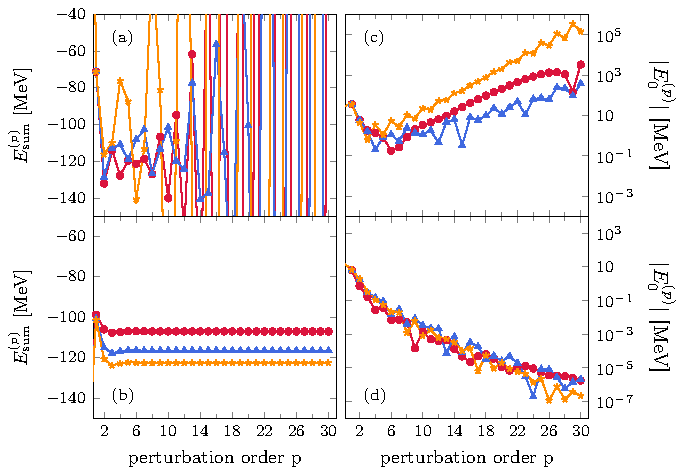
\includegraphics[width=0.8\textwidth]{proposal/doc/images/external/ho_vs_hf_mbpt.pdf}
  \caption[
    The partial sums (left) and order-by-order contributions (right)
    for an MBPT calculation of the ground-state energy of ${}^{16}\text{O}$
    using a harmonic-oscillator reference state (top)
    and a Hartree-Fock reference state (bottom).
    The red, blue, and yellow points are for $N_{\text{max}}=2$, 4, and 6,
    the basis truncation parameter for the approach used.
  ]{
    The partial sums (left) and order-by-order contributions (right)
    for an MBPT calculation of the ground-state energy of ${}^{16}\text{O}$
    using a harmonic-oscillator reference state (top)
    and a Hartree-Fock reference state (bottom).
    The red, blue, and yellow points are for $N_{\text{max}}=2$, 4, and 6,
    the basis truncation parameter for the approach used.
    Figure taken from Ref.~\cite{Tich16hohfmbpt}.
  }\label{fig:ho_vs_hf_mbpt}
\end{figure}

At the third order, even considering only canonical diagrams,
the number of diagrams possible with two- and three-body operators grows to 17.
The complete list of these diagrams can be found in Ref.~\cite{Hu18mbptthreebody}.
The canonical contributions involving only the normal-ordered two-body Hamiltonian are
\begin{equation}
  \begin{split}
  E^{(3)}_{\text{2-body only}} =
    &\frac{1}{8} \sum_{abcdij} \frac{\hnotwo_{ijab} \hnotwo_{abcd}\hnotwo_{cdij}}{\epsilon_{ij}^{ab}\epsilon_{ij}^{cd}} \\
    &+ \frac{1}{8} \sum_{abijkl} \frac{\hnotwo_{ijab} \hnotwo_{abkl}\hnotwo_{klij}}{\epsilon_{ij}^{ab}\epsilon_{kl}^{ab}} \\
    &- \sum_{abcijk} \frac{\hnotwo_{ijab} \hnotwo_{kbic}\hnotwo_{ackj}}{\epsilon_{ij}^{ab}\epsilon_{kj}^{ac}}\,.
  \end{split}
\end{equation}
The complete set of non-canonical third-order contributions
with only one- and two-body operators
is given, among other places, in Ref.~\cite{Tich17phd}.

The inclusion of additional terms is not the only challenge when dealing with a non-canonical reference state.
Choosing a different reference state than the HF determinant
corresponds to choosing a worse partitioning for $H$,
that is, more information is held in the perturbation $H_1$,
as the the HF determinant is the best possible single Slater determinant approximation
to the ground state.
This less optimal choice can lead to poor convergence behavior of MBPT~\cite{Tich16hohfmbpt}.
For instance, in Fig.~\ref{fig:ho_vs_hf_mbpt}
the ground-state energy of ${}^{16}\text{O}$ was calculated
using a harmonic-oscillator determinant and a Hartree-Fock determinant
for the reference state.
While for the HF reference state MBPT converges nicely,
for the HO reference state the calculation rapidly begins to diverge
when going to higher orders in perturbation theory.
Additionally,
while MBPT benefits strongly from working with SRG-evolved Hamiltonians,
it can have difficulty converging even when using an HF reference state
for bare nuclear Hamiltonians that are too ``hard''~\cite{Tich20mbptreview}.

\section{Non-perturbative techniques}

The convergence challenges of MBPT motivate us to consider non-perturbative many-body methods,
which sum to all orders certain types of diagrams to produce a convergent result.
Coupled cluster theory and the in-medium similarity renormalization group
are two examples of such methods.
Their non-perturbative nature makes them less sensitive to the choice of reference state
(although convergence speed will be affected by a non-canonical choice of reference state)
and better able to deal with ``harder'' nuclear Hamiltonians.
We discuss the IM-SRG in detail in the next chapter.
Here, we aim to briefly introduce the coupled cluster many-body approach
as it shares many similarities with the IM-SRG.\@

The ansatz for the coupled cluster (CC) approach is describing the ground state as
\begin{equation}
  \ket{\Psi} = \exp(T)\ket{\Phi}\,,
\end{equation}
where $T$ is the cluster operator,
which when applied exponentially to the reference state $\refgnd$ yields the ground state~\cite{Hage13ccreview}.
$T$ contains in general one- through $A$-body operators,
\begin{equation}
  T = \onebodyop{T} + \twobodyop{T} + \cdots + \abodyop{T}\,,
\end{equation}
which generate particle-hole excitations of the reference state.

The ground-state energy is then given by
\begin{align}
  E &= \braket{\Psi | H | \Psi} \\
  &= \braket{\Phi | \exp(-T) (\hnoone + \hnotwo + \hnothree) \exp(T) | \Phi} + \hnozero \\
  &\equiv \braket{\Phi | \overline{H} | \Phi} + \hnozero\,,
\end{align}
where we have defined the similarity-transformed Hamiltonian $\overline{H}$.
The task is to solve for matrix elements of the different $A$-body parts of $T$
such that
\begin{equation}
  0 = \braket{\Phi_{ijk\ldots}^{abc\ldots} | \overline{H} | \Phi}\,
\end{equation}
for all $n$-particle $n$-hole excited states of the reference state.
These are the coupled cluster equations.

One computes $\overline{H}$ via the Baker-Campbell-Hausdorff expansion,
\begin{equation}
  \overline{H} = H_N + \comm{H_N}{T} + \frac{1}{2!} \comm{\comm{H_N}{T}}{T} + \ldots \,,
\end{equation}
where $H_N=\hnoone + \hnotwo + \hnothree$.
This commutator expansion ensures that only connected diagrams in the MBPT expansion are generated,
ensuring the size-extensivity of the method.
A standard approach in nuclear physics is to truncate $T$, $H_N$, and the commutator
at the two-body level,
giving two coupled cluster equations
\begin{align}
  0 &= \braket{\Phi_{i}^{a} | \overline{H} | \Phi}\,,\\
  0 &= \braket{\Phi_{ij}^{ab} | \overline{H} | \Phi}\,,
\end{align}
known as CCSD (SD for singles and doubles).
Another variant approximately treats the so-called triples and is denoted CCSD(T).\@
In the next chapter, when discussing the IM-SRG,
the many similarities of the methods will be quite obvious.

